\documentclass[11pt]{article}
\usepackage[margin=1in]{geometry}
\usepackage[T1]{fontenc}
\usepackage{lmodern}
\usepackage{amsmath,amssymb,amsthm}
\usepackage{graphicx}
\usepackage{booktabs}
\usepackage[numbers,sort&compress]{natbib}
\usepackage{xcolor}
\usepackage[colorlinks=true,linkcolor=blue!50!black,citecolor=blue!50!black,urlcolor=blue!50!black]{hyperref}
\usepackage{enumitem}
\usepackage{microtype}

\newtheorem{proposition}{Proposition}
\newtheorem{lemma}{Lemma}
\newtheorem{definition}{Definition}
\theoremstyle{remark}
\newtheorem{remark}{Remark}
% Marks every number that still depends on a running experiment. Must be empty before submission.
\newcommand{\pending}[1]{\textcolor{red}{[#1]}}
\newcommand{\R}{\mathbb{R}}
\newcommand{\tr}{\operatorname{tr}}
\newcommand{\MS}{\operatorname{MS}}
\graphicspath{{../figures/}}

\title{Flat in the Wrong Coordinates:\\ Optimizer-Induced Symmetry Drift Biases\\ Sharpness Comparisons Between Adam and SGD}
\author{Ashvin J\\ School of Computer Science and Engineering, VIT-AP University\\ \texttt{ashvin.23bce8207@vitapstudent.ac.in}
% Add supervisor / co-authors here if appropriate.
}
\date{}

\begin{document}
\maketitle

\begin{abstract}
Empirical studies often compare how flat the minima found by different optimizers are, and the conclusions disagree. A preliminary version of this study used a common relative random-perturbation metric and found Adam's minima \emph{flatter} than SGD's on MNIST and CIFAR-10. We show that such comparisons mix two factors: the geometry of the learned function, and the point of the network's rescaling-symmetry orbit at which that function happens to be represented. For the Hessian trace the split is exact: raw trace $=$ \emph{minimum sharpness} (the trace minimized over function-preserving neuron rescalings) $\times$ \emph{orbit excess}. We prove that SGD's first-order drift along these orbits vanishes identically, whereas Adam's diagonal preconditioning moves it along them at first order. Empirically the drift scales as $\eta\sqrt{\text{fan-in}}$. Adam, and likewise RMSprop and sign descent, keeps its orbit excess low ($\approx1.2$ on MLPs, $1.4$--$1.8$ on a CNN) across hyperparameters and training stages. The excess of SGD, SGD with momentum and SAM is instead fixed by initialization and the conservation law, and reaches $3.4$. Across 162 loss-matched training runs and up to 17 measures, this coordinate factor is as large as the functional differences being measured. On a CIFAR-10 MLP it favours Adam by about $2\times$ and reverses the ordering: the probability that Adam is rated flatter than SGD is $0.62$--$0.75$ under coordinate-dependent trace measures but $0.01$--$0.22$ under minimum sharpness. On MNIST it flips the raw ordering in the middle of training. On a CNN, where Adam's solutions are clearly sharper at the function level, it hides most of the difference relative to SGD with momentum. Across MLPs with 1 to 8 hidden layers the coordinate factor stays at $1.4$--$1.8\times$ while Adam's function-level sharpness grows with depth, so the same factor reverses the ordering in shallow networks and masks it in deep ones. A causal intervention undoes Adam's drift after every step without changing the function. It roughly doubles raw trace-type sharpness at matched loss (median $\times1.9$ on CIFAR-10), leaves minimum sharpness unchanged ($\times0.98$), and removes Adam's apparent flatness advantage over SGD. In noisy regimes it also slows training, which suggests the drift helps Adam train. Moving SGD to the trace-minimizing coordinates instead (symmetry teleportation) destabilizes it: 10 of 16 teleported runs diverged, against none without teleports, because each teleport raised $\lambda_{\max}$ toward or above $2/\eta$. On long horizons with label noise, the orbit serves as a testbed for implicit sharpness regularization in a nonlinear network: SGD drifts toward the trace-minimizing point and Adam toward the minimizer of $\sum_i\sqrt{G_{ii}}$, the destinations predicted for each, in all 20 label-noise runs of each optimizer. Started from different points of the same orbit, both optimizers lose the initial difference in orbit excess within one epoch, yet Adam ends below SGD from every starting point. With BatchNorm the coordinate factor reverses the ordering in the opposite direction: raw measures follow learning-rate-dependent weight norms and rate Adam sharper, while measures invariant to every per-weight rescaling rate it flatter in all eight learning-rate pairings. Removing the coordinate factor also raises the cross-optimizer correlation between sharpness and generalization (Kendall $\tau$ $0.38\to0.61$ on CIFAR-10, $0.47\to0.62$ on MNIST) while leaving within-optimizer correlations unchanged. Re-running our original protocol shows that its ``Adam is flatter'' result came from this coordinate factor on CIFAR-10 and from a training-loss mismatch on MNIST. We recommend that cross-optimizer flatness comparisons report rescaling-invariant measures, or at least the orbit excess.
\end{abstract}

%===============================================================================
\section{Introduction}
%===============================================================================
The idea that flat minima generalize better than sharp ones \citep{hochreiter1997flat,keskar2017large} motivates both analysis tools and optimizers such as SAM \citep{foret2021sam}. A recurring empirical question is \emph{which optimizer finds flatter minima}. Adaptive methods such as Adam \citep{kingma2015adam} are often reported to generalize worse than SGD \citep{wilson2017marginal}, and a popular explanation is that they converge to sharper minima \citep{zhou2020towards}. Measurements nevertheless disagree, and recent theory suggests that Adam and SGD implicitly minimize \emph{different} notions of sharpness \citep{li2025adam}.

This paper began as an attempt to answer that question with a standard tool, the relative increase in loss under isotropic Gaussian weight noise, $(L(w+\sigma\varepsilon)-L(w))/L(w)$. The preliminary result was that Adam's minima appeared \emph{flatter} than SGD's on both MNIST and CIFAR-10, the opposite of the usual narrative. Before reporting it, we checked whether it was an artifact. It was, and the reason turned out to be general and mechanistic.

Coordinate-dependent sharpness is known to be manipulable: \citet{dinh2017sharp} showed that function-preserving reparameterizations of ReLU networks can make any minimum arbitrarily sharp or flat. A common reply is that no optimizer performs such reparameterizations, so the objection is academic. Our central finding is that \textbf{Adam does perform them}. It moves systematically along the network's rescaling symmetries and settles near the coordinates in which its solution has the smallest possible Hessian trace. SGD provably does not move along them at first order. A raw sharpness comparison between Adam and SGD therefore compares two functions \emph{and} two positions on their symmetry orbits, and we show that the second factor is often the larger one. Figure~\ref{fig:teaser} illustrates this on two trained CIFAR-10 networks.

\begin{figure}[t]
\centering
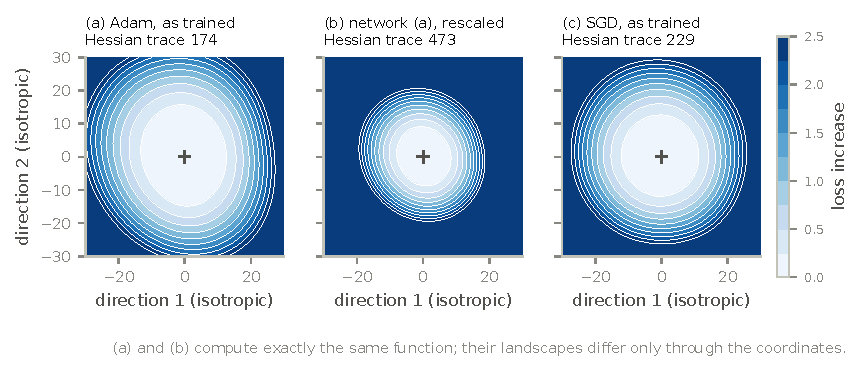
\includegraphics[width=0.95\linewidth]{fig0_same_function.pdf}
\caption{\textbf{Same function, different landscape.} Two-dimensional loss slices along the same two random isotropic directions around (a) an MLP trained with Adam, (b) the \emph{identical function} obtained from (a) by rescaling each hidden neuron's incoming and outgoing weights (to the minimum-norm representative), and (c) an MLP trained with SGD. All three are at training loss $\le0.01$ on CIFAR-10. By the isotropic picture, or its Hessian trace, Adam's solution looks flatter than SGD's, yet a function-preserving change of coordinates makes it look $2.7\times$ sharper. Adam's training dynamics drift toward coordinates like (a); SGD's cannot (\S\ref{sec:mechanism}).}
\label{fig:teaser}
\end{figure}

\paragraph{Contributions.}
\begin{itemize}[leftmargin=1.2em,itemsep=2pt]
\item \textbf{An exact decomposition} (\S\ref{sec:setup}). The Hessian (Gauss--Newton) trace factors into the minimum sharpness of the function \citep{ibayashi2021minimum} times an orbit excess $\ge1$ that depends only on the representation. Both factors are cheap to compute exactly.
\item \textbf{A mechanism with a proof and a scaling law} (\S\ref{sec:mechanism}). The first-order drift of the per-unit conserved quantity $\|w_{\mathrm{in}}\|^2-\|w_{\mathrm{out}}\|^2$ vanishes identically for SGD, is second order for heavy-ball momentum, and is generically nonzero for diagonally preconditioned methods. For sign-like updates it scales with the units' $\ell_1$ norms, which predicts the $\eta\sqrt{\text{fan-in}}$ law we measure (fitted exponents $0.91$ and $0.94$).
\item \textbf{A loss-matched, multi-measure audit} (\S\ref{sec:audit}). We compare SGD, SGD+momentum, SAM and Adam at \emph{matched training loss} on MLPs (MNIST, CIFAR-10) and a CNN (CIFAR-10), using 17 measures. Adam keeps a low orbit excess ($\approx1.2$ on the MLPs, $1.4$--$1.8$ on the CNN) while the other optimizers reach $3.4$. Depending on the size of the true functional difference, this coordinate factor reverses the optimizer ranking (CIFAR-10 MLP), flips it during training (MNIST), or masks a large difference (CNN). It does not grow with depth (\S\ref{sec:depth}).
\item \textbf{A causal test} (\S\ref{sec:intervention}). \emph{Adam-Q} applies, after each Adam step, the function-preserving rescaling that undoes the drift. At matched training loss it isolates the coordinate effect: raw sharpness roughly doubles while invariant sharpness is unchanged. In noisy regimes Adam-Q also trains more slowly, a hint that the drift matters for optimization as well as for measurement.
\item \textbf{A two-phase picture of orbit dynamics} (\S\ref{sec:mechanism}, \S\ref{sec:teleport}, \S\ref{sec:labelnoise}). Adam's first-order drift takes it close to the trace-minimizing point within a few epochs. A slower, noise-driven drift then moves SGD toward minimum trace and Adam toward minimum $\sum_i\sqrt{G_{ii}}$, which we confirm with label noise in all 20 runs of each optimizer across two experiments. Starting the same function at different orbit points shows that the excess is set by training dynamics rather than inherited from initialization, and that Adam's lower excess holds from every start. Adam's coordinates do not help SGD: teleporting SGD to them raises $\lambda_{\max}$ toward $2/\eta$, and most teleported runs diverge.
\item \textbf{Consequences} (\S\ref{sec:generalization}, \S\ref{sec:replication}, \S\ref{sec:bn}). The coordinate factor specifically degrades \emph{cross-optimizer} sharpness--generalization correlations, and it explains (together with a loss-level confound) our original result. With BatchNorm, raw measures are dominated by learning-rate-dependent weight norms, and the raw ordering is set by the learning-rate pairing while invariant measures give one consistent verdict.
\end{itemize}

%===============================================================================
\section{Related work}
%===============================================================================
\paragraph{Sharpness and generalization.} Many measures exist: worst-case and average-case perturbation sharpness \citep{keskar2017large,jiang2020fantastic}, the Hessian trace and top eigenvalue, and adaptive or normalized variants designed for scale invariance \citep{kwon2021asam,tsuzuku2020normalized,petzka2021relative,rangamani2019scale,li2018visualizing}. Large-scale studies find that their correlation with generalization is fragile \citep{jiang2020fantastic,andriushchenko2023modern,kaur2023maximum}. \citet{dinh2017sharp} exhibited reparameterizations that change sharpness arbitrarily without changing the function. \citet{ibayashi2021minimum} proposed \emph{minimum sharpness}, the minimal Hessian trace over rescaling-equivalent parameterizations, and reported that it correlates well with generalization. We use their quantity, generalize it to other powers of the curvature and to conv nets, and show that the gap between raw trace and minimum sharpness is systematically \emph{optimizer-dependent}. \citet{zhang2021flatness} observed that Adam can break the correlation between flatness and generalization, and proposed a parameterization-invariant Bayesian alternative. We identify a concrete mechanism behind such breakdowns and measure its size.

\paragraph{Symmetries and conservation laws.} Gradient flow on homogeneous networks conserves $\|w_{\mathrm{in}}\|^2-\|w_{\mathrm{out}}\|^2$ per unit \citep{du2018algorithmic}. Path-SGD \citep{neyshabur2015path} was designed to make optimization itself invariant to these rescalings. \citet{kunin2021neural} analysed how finite learning rates, momentum and weight decay break such laws. \citet{marcotte2023abide,marcotte2024keep} characterized conservation laws for gradient flows and showed that none survive momentum dynamics in ReLU networks. \citet{ziyin2023law,ziyin2024parameter} showed that SGD's minibatch noise slowly moves parameters along rescaling and other exponential symmetries toward a ``noise equilibrium''. This is a second-order effect, consistent with Proposition~\ref{prop:drift}a. Closest to our mechanism, \citet{singh2026loss} showed that gradient descent, momentum, Shampoo and Muon are equivariant under the gauge symmetry of matrix factorization while coordinate-wise methods (Adam, RMSProp, signum) are not, and that this changes which interpolant is found. Our Proposition~\ref{prop:drift} is the analogous statement for the ReLU rescaling symmetry. Symmetry \emph{teleportation} \citep{zhao2022teleport,zhao2024improving} moves parameters along orbits deliberately, to speed up optimization or to reach minima of different curvature. Our contribution is not that adaptive methods break these symmetries, which follows from the work above. It is to show where the drift leads (near minimum sharpness), to measure how large it is ($\eta\sqrt{\text{fan-in}}$; a factor $\approx2$ in the Hessian trace), and to show that it biases flatness comparisons between optimizers enough to reverse, flip or mask them.

\paragraph{Implicit sharpness regularization.} SGD with label noise implicitly minimizes $\tr H$ near the minimizer manifold \citep{blanc2020implicit,damian2021label}, and \citet{li2025adam} prove that Adam instead minimizes $\tr\,\mathrm{diag}(H)^{1/2}$. Gradient methods train at the edge of stability \citep{cohen2021eos,cohen2022adaptive}, so their sharpness is largely set by the learning rate. We see this too (Appendix~\ref{app:eos}), which is why we compare optimizers over many learning rates rather than at one.

%===============================================================================
\section{Rescaling orbits, a conservation law, and minimum sharpness}\label{sec:setup}
%===============================================================================
Consider a network built from linear (or convolutional) layers and positively homogeneous activations (ReLU, max-pooling). For a hidden unit $j$ (a neuron, or a convolutional channel) let $a_j$ collect its incoming weights and bias and $c_j$ its outgoing weights. For $s\in\R$, the map $T^{(j)}_s:(a_j,c_j)\mapsto(e^{s}a_j,\,e^{-s}c_j)$ leaves the network function unchanged. Applying such maps to all units generates the \emph{rescaling orbit} of $\theta$.

\begin{lemma}[Euler identity]\label{lem:euler}
For any loss $\ell$ that depends on $\theta$ only through the network function, including any minibatch loss, $\langle a_j,\nabla_{a_j}\ell\rangle=\langle c_j,\nabla_{c_j}\ell\rangle$ for every hidden unit $j$.
\end{lemma}
\begin{proof}
$s\mapsto\ell(T^{(j)}_s\theta)$ is constant; differentiate at $s=0$.
\end{proof}

Let $Q_j=\|a_j\|^2-\|c_j\|^2$. Lemma~\ref{lem:euler} gives $\dot Q_j=0$ under gradient flow \citep{du2018algorithmic}. For a discrete update $\theta^+=\theta+u$, expanding $\|a+u_a\|^2$ gives the \emph{exact} decomposition
\begin{equation}\label{eq:decomp}
Q_j(\theta^+)-Q_j(\theta)=\underbrace{2\big(\langle a_j,u_{a_j}\rangle-\langle c_j,u_{c_j}\rangle\big)}_{D^{(1)}_j\ \text{(first order)}}+\underbrace{\|u_{a_j}\|^2-\|u_{c_j}\|^2}_{D^{(2)}_j\ \text{(second order)}}.
\end{equation}

\begin{proposition}\label{prop:drift}
\textbf{(a) SGD.} For $u=-\eta\nabla\ell_B$ on any minibatch $B$, $D^{(1)}_j=0$ exactly and $D^{(2)}_j=\eta^2(\|\nabla_{a_j}\ell_B\|^2-\|\nabla_{c_j}\ell_B\|^2)$.
\textbf{(b) Heavy-ball momentum.} For $u_t=-\eta\sum_{k\ge0}\beta^k g_{t-k}$,
$D^{(1)}_j=-2\eta\sum_k\beta^k\big(\langle a_{j,t}-a_{j,t-k},g_{a,t-k}\rangle-\langle c_{j,t}-c_{j,t-k},g_{c,t-k}\rangle\big)$.
Each term contains a parameter difference, which is itself $O(\eta)$, so the drift is again second order in $\eta$.
\textbf{(c) Diagonal preconditioning (Adam, RMSProp, sign descent).} For $u=-\eta P^{-1}m$ with diagonal $P\succ0$,
$D^{(1)}_j=-2\eta\big(\langle a_j,P_a^{-1}m_a\rangle-\langle c_j,P_c^{-1}m_c\rangle\big)$, which is generically nonzero. For sign descent, $u=-\eta\,\mathrm{sign}(g)$, this gives $D^{(1)}_j=2\eta\big(\rho_{a}\|a_j\|_1-\rho_{c}\|c_j\|_1\big)$, where $\rho_x=-\langle x,\mathrm{sign}(g_x)\rangle/\|x\|_1\in[-1,1]$ is the $\ell_1$-weighted net fraction of coordinates moving away from zero.
\end{proposition}
\begin{proof}
(a) Lemma~\ref{lem:euler} applied to $\ell_B$. (b) Apply Lemma~\ref{lem:euler} at time $t-k$ to $g_{t-k}$ and subtract. (c) Direct substitution.
\end{proof}

\begin{remark}[Why the drift scales with $\sqrt{\text{fan-in}}$]\label{rem:fanin}
SGD moves each weight in proportion to the magnitude of its partner weights, and this is what keeps $Q_j$ fixed. Sign-like updates move every coordinate by about $\eta$ whatever its magnitude. During norm growth ($\rho>0$), the side with the larger $\ell_1$ norm therefore gains squared norm faster. For dense vectors $\|x\|_1\approx\kappa\sqrt{d}\,\|x\|_2$ ($\kappa=\sqrt{2/\pi}$ for Gaussian entries), so a unit whose fan-in exceeds its fan-out drifts toward large incoming norm at a rate $\propto\eta\sqrt{d_{\mathrm{in}}}$. Adam behaves like sign descent when gradient noise is small relative to the signal \citep{balles2018dissecting,bernstein2018signsgd}.
\end{remark}

\paragraph{Exact transport of curvature along the orbit.} A rescaling acts linearly, $\theta'=D\theta$ with $D$ diagonal and positive. The Hessian and the Gauss--Newton matrix $G$ \citep{martens2020new} therefore transform \emph{exactly} as $H(\theta')=D^{-1}H(\theta)D^{-1}$, so $\mathrm{diag}(G)$ anywhere on the orbit follows from $\mathrm{diag}(G)$ at $\theta$ in closed form.

\begin{definition}[Minimum sharpness and orbit excess]
Following \citet{ibayashi2021minimum}, and generalizing to powers $p>0$,
$\MS_p(\theta)=\min_{\theta'\in\mathrm{orbit}(\theta)}\sum_iG_{ii}(\theta')^{p}$.
$\MS_1$ is the minimal trace; $\MS_{1/2}$ is the minimum of the regularizer that Adam implicitly minimizes \citep{li2025adam}. The \emph{orbit excess} is $E(\theta)=\tr G(\theta)/\MS_1(\theta)\ge1$, so that
\begin{equation}\label{eq:factor}
\tr G(\theta)=\underbrace{\MS_1(\theta)}_{\text{function}}\times\underbrace{E(\theta)}_{\text{coordinates}}.
\end{equation}
\end{definition}

$\MS_1$ is constant on the orbit, so it depends only on the function. $E$ measures how far the current coordinates are from the flattest representation. Comparing two networks in $\log\tr G$ therefore splits \emph{exactly} into a function term and a coordinate term. A weight rescaled by $s$ contributes $G_{ii}^p s^{-2p}$, so the objective is a posynomial in the unit scales and is convex in their logarithms. Exact coordinate descent has a closed form: unit $j$ sees $A_jc_j^{-2p}+B_jc_j^{2p}$, minimized at $c_j^{2p}=\sqrt{A_j/B_j}$, where $A_j$ and $B_j$ aggregate its incoming and outgoing curvature. At $p=1$ the optimum is characterized by \emph{curvature balance}, with equal incoming and outgoing curvature for every unit. This differs from the minimum-norm (``balanced'') point, where incoming and outgoing \emph{norms} are equal. We compute $\mathrm{diag}(G)$ exactly. For MLPs, one backward pass per class suffices, accumulating $\sum_n p_{nk}(\delta_{nk}^2)^\top(a_n^2)$ per layer; for CNNs we use per-sample gradients. After that, $\MS_p$ takes milliseconds.

%===============================================================================
\section{Experimental protocol}\label{sec:protocol}
%===============================================================================
\textbf{Data and models.} We use MNIST and CIFAR-10 with a class-balanced 10k-example training subset, the full test set, and per-channel input standardization. The models are an MLP in--128--64--10 (the architecture of the original study) and a small CNN (two $3{\times}3$ conv layers with 32 and 64 channels, each followed by $2{\times}2$ max-pooling, then FC 128 and FC 10). Neither has normalization layers.
\textbf{Optimizers.} SGD, SGD with momentum $0.9$ (SGD+M), SAM ($\rho=0.05$, SGD+M base) and Adam (default $\beta$s, $\epsilon=10^{-8}$). For each optimizer we use two base learning rates and batch sizes $\{32,128,512\}$ with square-root scaling $\eta=\eta_0\sqrt{B/32}$, and three seeds, for 72 runs per dataset. A calibration sweep chose the base rates so that every configuration trains stably (Appendix~\ref{app:calibration}).
\textbf{Loss matching.} Comparing optimizers after a fixed number of epochs conflates optimizer effects with how far training has progressed, and cross-entropy curvature shrinks with the loss. Each run is therefore measured when its full training loss first falls below each of $\{1,0.3,0.1,0.03,0.01\}$, and only checkpoints at the same target are compared. All 144 MLP runs reached every target. (One CIFAR-10 SGD+M run crossed $0.03$ and $0.01$ within the same epoch; its checkpoint is used for $0.01$ only.)
\textbf{Measures.} On a fixed subset of 4096 training examples we compute 17 measures (Appendix~\ref{app:measures}).
\emph{Coordinate-dependent:} the original metric (relative isotropic Gaussian sharpness on the test set, $\sigma=0.01$); isotropic average sharpness; the Hessian trace (Hutchinson, \citealp{hutchinson1989stochastic}) and exact $\tr G$; $\lambda_{\max}$ (Lanczos); worst-case SAM sharpness (10-step PGD); $\sum_i\sqrt{G_{ii}}$; and several of these at the minimum-norm point (\emph{canonicalized}).
\emph{Rescaling-invariant:} $\MS_1$, $\MS_{1/2}$, multiplicative (elementwise-relative) average sharpness, ASAM worst-case sharpness \citep{kwon2021asam}, and $\sum_iw_i^2G_{ii}$. We also report filter-normalized average sharpness \citep{li2018visualizing}, which is often used as a scale-invariant measure. It is invariant to scaling a unit's incoming weights, but \emph{not} to the compensating scaling of its outgoing weights, which changes the norms of the next layer's rows unevenly. A random rescaling with log-scale s.d.\ $1$ changes it by a factor of $9.5$ in our MLP, while the other perturbation measures above are unchanged to within $10^{-4}$ (\texttt{scripts/test\_invariance.py}). We therefore treat it as \emph{partially} invariant.
\textbf{Statistic.} For a measure $S$ we report $P(S_{\mathrm{Adam}}<S_X)$ over all pairs of Adam and $X$ configurations sharing a seed and loss target (108 pairs). This is a common-language effect size, with $0.5$ meaning no difference. For the trace we also report the exact split of $\log_2(\overline{\tr G}_{\mathrm{Adam}}/\overline{\tr G}_X)$ (geometric means) into function and coordinate terms via~\eqref{eq:factor}. 95\% confidence intervals come from a cluster bootstrap that resamples runs within each seed (2000 resamples).

%===============================================================================
\section{Results}
%===============================================================================
\subsection{Adam drifts along the orbit; SGD does not}\label{sec:mechanism}
\begin{figure}[t]
\centering
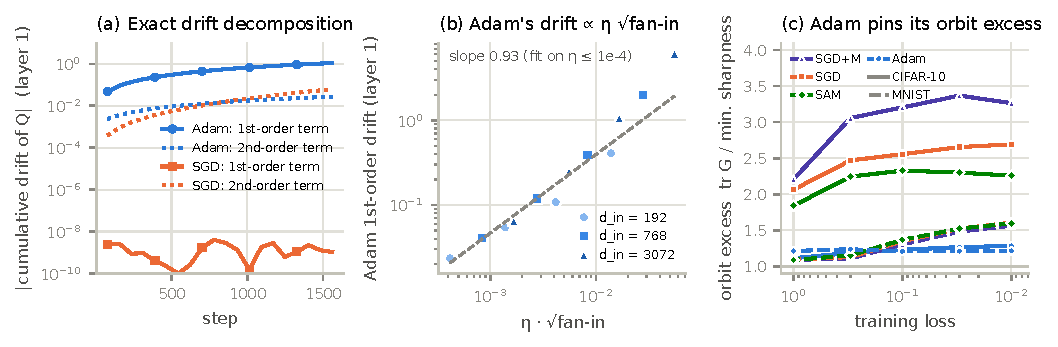
\includegraphics[width=\linewidth]{fig2_mechanism.pdf}
\caption{\textbf{(a)} Exact decomposition~\eqref{eq:decomp} of the cumulative drift of $Q_j$ (mean over first-layer units; CIFAR-10 MLP, $32{\times}32$ inputs). SGD's first-order term is zero up to float32 round-off ($\sim10^{-9}$), as Proposition~\ref{prop:drift}a requires, while Adam's first-order term dominates its own second-order term. \textbf{(b)} Adam's first-order drift after 20 epochs, for four learning rates and three input resolutions (fan-in 192, 768 and 3072), plotted against $\eta\sqrt{\text{fan-in}}$. \textbf{(c)} Orbit excess $E=\tr G/\MS_1$ at matched training loss (median of 18 runs; solid: CIFAR-10, dashed: MNIST). Adam holds $E\approx1.2$ on both datasets; the other optimizers' excess depends on dataset and training stage.}
\label{fig:mechanism}
\end{figure}

We first isolate the mechanism. We log both terms of~\eqref{eq:decomp} at every step on the CIFAR-10 MLP, varying the learning rate ($3{\times}10^{-5}$--$10^{-3}$ for Adam, $0.01$--$0.1$ for SGD, $10^{-3}$--$10^{-2}$ for SGD+M) and the first layer's fan-in (inputs average-pooled to $8{\times}8$, $16{\times}16$ and $32{\times}32$), with two seeds per setting (66 runs). The decomposition closes to $\le1.3{\times}10^{-6}$ (float32 round-off) in every run.

\textbf{SGD conserves; Adam drifts.} SGD's first-order term is below $3{\times}10^{-7}$ in every run, zero up to round-off as Proposition~\ref{prop:drift}a requires. Adam's is $0.02$--$6.2$, five to seven orders of magnitude larger, and exceeds its own second-order term by $23$--$800\times$ (Fig.~\ref{fig:mechanism}a). SGD+M drifts only at second order, as Proposition~\ref{prop:drift}b predicts. At equal effective learning rate $\eta/(1-\beta)$ its total drift matches SGD's ($0.61$ vs.\ $0.58$ at $\eta_{\mathrm{eff}}=0.1$, $32{\times}32$).

\textbf{Scaling law.} A log-linear fit of Adam's first-layer first-order drift on $\log\eta$ and $\log\sqrt{d_{\mathrm{in}}}$ gives exponents $0.91$ and $0.94$ for $\eta\le10^{-4}$, close to the $\eta\sqrt{d_{\mathrm{in}}}$ predicted by Remark~\ref{rem:fanin} (Fig.~\ref{fig:mechanism}b). Over all learning rates the fit gives $1.07$ and $1.38$ ($R^2=0.97$). The steeper fan-in dependence at large $\eta$ is consistent with the remark, since the $\ell_1$ norms that drive the drift keep growing as training progresses further. The drift of the second layer, whose fan-in is fixed at 128, does not depend on input resolution. Seeds agree to within a few percent.

\textbf{Where the drift leads.} At initialization the CIFAR-10 MLP has orbit excess $E=3.66$; MNIST has $1.79$. During training, Adam moves to a median $E=1.11$--$1.28$ on CIFAR-10 and $1.21$--$1.24$ on MNIST, at every loss level (Fig.~\ref{fig:mechanism}c). Across all 90 Adam checkpoints, $E$ lies in $[1.08,1.48]$ on CIFAR-10, against $[1.45,4.89]$ for the other optimizers, and in $[1.12,1.48]$ on MNIST. As the $\eta$-proportional drift predicts, the excess is slightly higher at Adam's smaller base learning rate (CIFAR-10 median $1.29$--$1.38$ vs.\ $1.15$--$1.17$), where there is less drift to carry the network away from its initial coordinates. SGD, SGD+M and SAM cannot move along the orbit at first order, so their excess follows from their conserved $Q_j$ combined with how the curvature redistributes during training; the second factor dominates, and SGD reaches a similar excess from very different starting points (\S\ref{sec:labelnoise}). Their median excess is $1.8$--$3.4$ on CIFAR-10 and drifts from $1.1$ to $1.6$ on MNIST. In parameter space, Adam's first-layer imbalance $|\log(\|a_j\|/\|c_j\|)|$ reaches $0.82$--$1.07$ on CIFAR-10 (an incoming/outgoing norm ratio of about $2.9$), compared with $0.30$--$0.46$ for the other optimizers, which stay near the initial $0.35$.

\textbf{Not specific to Adam.} Proposition~\ref{prop:drift}c covers every diagonal preconditioner. Repeating the drift experiment with RMSprop and with plain sign descent (signSGD, which has neither momentum nor second-moment estimates) gives the same picture (Table~\ref{tab:drift}). Both drift at first order, and with $32{\times}32$ inputs all three adaptive methods end at an orbit excess of $1.10$--$1.28$, against $1.68$--$2.41$ for SGD and SGD+M at comparable training losses. The common ingredient is that every coordinate takes a step of roughly the same size.

\paragraph{Where the drift leads: two phases.} The data and the theory point to two distinct phases.

\emph{Noise-driven phase (slow).} SGD is not standing still on the orbit. Its second-order term has expectation $\mathbb{E}D^{(2)}_j=\eta^2(\mathbb{E}\|g_{a_j}\|^2-\mathbb{E}\|g_{c_j}\|^2)$. Near a minimum, minibatch gradients are dominated by noise and the Fisher matrix approximates the Gauss--Newton matrix, so this is approximately $\frac{\eta^2}{B}(A_j-B_j)$. Here $A_j=\sum_{i\in\mathrm{in}(j)}G_{ii}$ and $B_j=\sum_{k\in\mathrm{out}(j)}G_{kk}$ are the unit's incoming and outgoing curvature. A positive drift enlarges the incoming weights, which lowers $A_j$ ($\propto c_j^{-2}$) and raises $B_j$ ($\propto c_j^{2}$). The drift therefore pushes every unit toward \emph{curvature balance} $A_j=B_j$, the stationarity condition of $\MS_1$. This is the ``law of balance'' of \citet{ziyin2023law,ziyin2024parameter} written in curvature terms, and the orbit component of the $\tr H$-minimizing implicit bias of label-noise SGD \citep{blanc2020implicit,damian2021label}; see also implicit gradient regularization \citep{barrett2021implicit}.

The same argument can be applied to Adam. For a quasi-static diagonal preconditioner $P$, Adam's update is an SGD step in the coordinates $\theta'=P^{1/2}\theta$. Because $P$ is diagonal it commutes with the rescaling, so Lemma~\ref{lem:euler} still holds in $\theta'$. The noise covariance in these coordinates is $P^{-1/2}\Sigma P^{-1/2}$. With $p_i\approx\sqrt{\mathbb{E}g_i^2}$, noise balance then requires $\sum_{\mathrm{in}}\sqrt{\Sigma_{ii}}=\sum_{\mathrm{out}}\sqrt{\Sigma_{kk}}$, i.e.\ $\sum_{\mathrm{in}}\sqrt{G_{ii}}=\sum_{\mathrm{out}}\sqrt{G_{kk}}$. That is the stationarity condition of $\MS_{1/2}$, the orbit restriction of the $\tr\,\mathrm{diag}(H)^{1/2}$ regularizer that \citet{li2025adam} derive rigorously for Adam. The heuristic therefore predicts \emph{different} long-run destinations: minimum trace for SGD and minimum $\sum_i\sqrt{G_{ii}}$ for Adam, both reached at $O(\eta^2)$ per step.

\emph{Signal-driven phase (fast).} Early in training the gradient has a large mean, and Adam's first-order term (Proposition~\ref{prop:drift}c) dominates. Empirically it takes Adam from an orbit excess of about $3.7$ at initialization to $\approx1.1$ within about five epochs on CIFAR-10 (\S\ref{sec:labelnoise}), i.e.\ close to the trace-minimizing point. We have only a heuristic for this destination. Adam's per-coordinate steps have roughly equal size $\eta$ whatever the curvature, so the loss injected by its update noise, $\approx\frac{\eta^2}{2}\sum_iH_{ii}r_i^2$ with $r_i$ roughly constant, is proportional to $\tr H$ in the current coordinates. SGD has no first-order drift, so in this phase it stays wherever its initialization and its conserved $Q_j$ put it.

Ordinary training, and every optimizer comparison in \S\ref{sec:audit}, lives in the regime where the fast phase has acted and the slow phase has not. \S\ref{sec:labelnoise} tests both phases directly.

\subsection{Consequence: the coordinate factor reverses optimizer rankings}\label{sec:audit}
\begin{figure}[t]
\centering
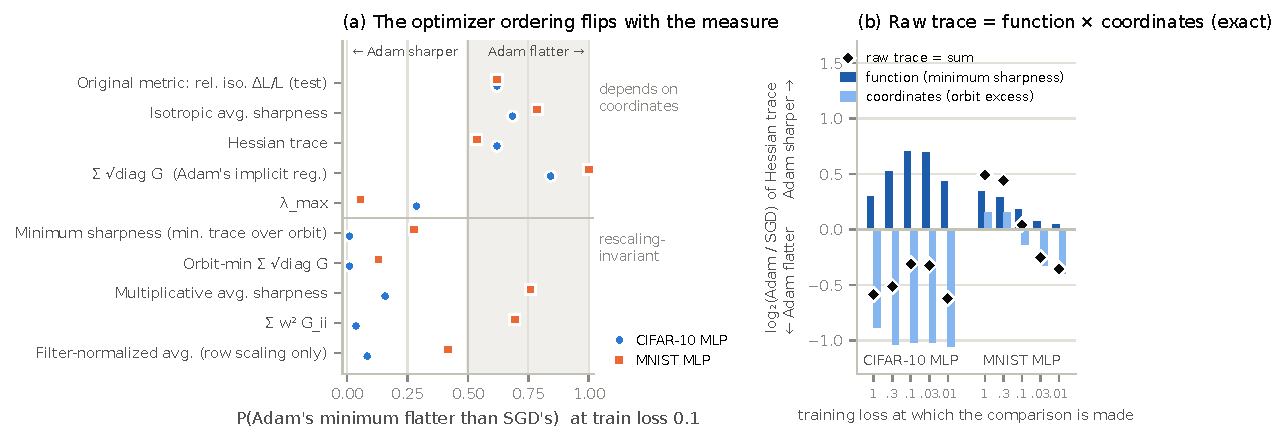
\includegraphics[width=\linewidth]{fig1_flip.pdf}
\caption{\textbf{(a)} Probability that Adam's minimum is rated flatter than SGD's, over all 108 loss-matched configuration pairs at training loss $0.1$. \textbf{(b)} Exact split~\eqref{eq:factor} of the Adam/SGD ratio of Hessian (Gauss--Newton) traces into a function term (minimum sharpness) and a coordinate term (orbit excess), at each matched training loss. On CIFAR-10, the coordinate term favours Adam by $\approx2\times$ and outweighs the function term, which favours SGD. On MNIST, the coordinate term changes sign during training and flips the raw ordering, while the function term never favours Adam.}
\label{fig:flip}
\end{figure}

\paragraph{CIFAR-10.} Figure~\ref{fig:flip} and Table~\ref{tab:flip} summarize the audit. At every matched training loss, Adam is rated flatter than SGD by the original metric ($P=0.62$--$0.67$), isotropic average sharpness ($0.69$--$0.75$), the Hessian trace ($0.62$--$0.74$) and, most strongly, $\sum_i\sqrt{G_{ii}}$ ($0.84$--$1.00$). Minimum sharpness reverses the conclusion ($P=0.01$--$0.22$), as do $\MS_{1/2}$ ($0.01$--$0.19$), filter-normalized sharpness ($0.06$--$0.14$), multiplicative sharpness ($0.16$--$0.31$) and $\sum w_i^2G_{ii}$ ($0.04$--$0.24$). With 18 runs per optimizer the raw verdicts carry substantial uncertainty (e.g.\ $\tr G$ at loss $0.1$: $P=0.64$, 95\% CI $[0.44,0.83]$), whereas the invariant verdicts are tight ($\MS_1$: $0.01$, $[0.00,0.06]$). The quantity that matters, the disagreement between them, is well determined: $P_{\tr G}-P_{\MS_1}=+0.69$ $[+0.52,+0.83]$, $+0.63$ $[+0.43,+0.81]$ and $+0.50$ $[+0.34,+0.67]$ at losses $0.3$, $0.1$ and $0.01$. The exact split explains this. In bits, $\log_2(\tr G_{\mathrm{Adam}}/\tr G_{\mathrm{SGD}})$ decomposes into a function term of $+0.52$ $[+0.36,+0.68]$, $+0.71$ $[+0.53,+0.87]$ and $+0.43$ $[+0.16,+0.71]$ (Adam sharper), and a coordinate term of $-1.03$ $[-1.17,-0.91]$, $-1.02$ $[-1.16,-0.87]$ and $-1.05$ $[-1.22,-0.89]$, a factor of almost exactly $2$ in Adam's favour at every loss level. Against SGD+M the coordinate term is larger still ($-0.94$ to $-1.33$ bits). Against SAM, the one optimizer designed to seek flat minima, the raw trace is inconclusive ($P=0.44$--$0.60$) because a large function term ($+0.69$ to $+1.00$ bits, SAM flatter) is cancelled by the coordinate term ($-0.69$ to $-0.92$). Invariant measures identify SAM as clearly flatter ($P=0.00$--$0.23$). A measure that fails this sanity check should not be used to rank optimizers.

\textbf{Robustness to the learning-rate pairing.} Sharpness depends strongly on the learning rate, so we also split the comparison by the pair of base learning rates (Table~\ref{tab:lrpairs}, pooled over batch sizes, seeds and losses $0.1$--$0.01$). On CIFAR-10 the raw verdict is set by the pairing: $P$ for $\tr G$ is $1.00$, $0.06$, $1.00$ and $0.60$ in the four pairings, and the original metric ranges from $0.00$ to $1.00$. Minimum sharpness rates Adam sharper in all four pairings ($P\le0.27$), and so does filter-normalized sharpness ($P\le0.09$). On MNIST both raw and invariant verdicts depend on the pairing ($\MS_1$: $0.00$--$0.88$), consistent with the small functional differences there.

\paragraph{MNIST.} Here the initial excess is smaller and the picture shifts during training (Fig.~\ref{fig:flip}b). Early on (training loss $1$ to $0.3$), SGD's excess is \emph{below} Adam's. The coordinate term therefore slightly favours SGD ($+0.15$ $[+0.12,+0.19]$ bits at loss $0.3$), and raw measures rate Adam sharper ($P=0.06$ for the trace). As SGD's excess grows, the coordinate term turns in Adam's favour ($-0.40$ $[-0.41,-0.38]$ bits at loss $0.01$) and the raw trace ordering flips ($P=0.80$, $[0.63,0.94]$). The original metric goes from $0.27$ to $0.97$. The function term never favours Adam: it shrinks from $+0.34$ to $+0.04$ bits (the latter indistinguishable from zero, $[-0.13,+0.22]$), and minimum sharpness gives $P=0.09$, $0.28$ and $0.44$ at losses $0.3$, $0.1$ and $0.01$. On MNIST, then, whether ``Adam is flatter'' depends on \emph{when} one measures, and the dependence comes almost entirely from the coordinate factor.

\paragraph{Invariant measures need not agree with each other.} Invariance removes the coordinate artifact, but it does not make different notions of flatness coincide. On CIFAR-10 all invariant measures agree, with one exception: large-radius ASAM at the earliest target ($P=0.71$ at loss $0.3$, then $0.32$ and $0.28$). On MNIST, the elementwise-relative family (multiplicative sharpness, ASAM, $\sum_iw_i^2G_{ii}$) rates Adam flatter late in training ($P=0.73$--$0.87$ at loss $0.01$), while minimum sharpness and filter-normalized sharpness do not ($0.44$ and $0.20$). The relative measures weight each weight's curvature by its squared magnitude, which is itself affected by Adam's sign-like updates. We therefore make no universal claim that Adam's minima \emph{are} sharper. Our claim is narrower and robust: the raw-coordinate ordering is biased by an optimizer-dependent factor that is as large as the effects being measured.

\paragraph{$\lambda_{\max}$ and canonicalization.} The top eigenvalue rates Adam sharper even in raw coordinates ($P=0.29$--$0.45$ on CIFAR-10, $0.00$--$0.32$ on MNIST), in line with prior reports and with edge-of-stability dynamics. It is dominated by a few outlier directions, while the drift mainly reshapes the bulk of the diagonal that trace-type and isotropic measures integrate. Mapping each network to its minimum-norm representative before measuring only partly removes the bias ($P=0.31$--$0.56$ for the trace on CIFAR-10). Adam's drift moves toward \emph{curvature} balance, which is the condition for minimum sharpness, not toward norm balance.

\begin{table}[t]
\centering
\small
\caption{$P(\text{Adam rated flatter than }X)$ at matched training loss $L$ (108 configuration pairs per cell). Values below $0.5$ mean Adam is rated sharper.}
\label{tab:flip}
\setlength{\tabcolsep}{4pt}
\begin{tabular}{llccccccccc}
\toprule
& & \multicolumn{3}{c}{CIFAR-10, vs SGD} & \multicolumn{3}{c}{CIFAR-10, vs SAM} & \multicolumn{3}{c}{MNIST, vs SGD}\\
\cmidrule(lr){3-5}\cmidrule(lr){6-8}\cmidrule(lr){9-11}
Measure & type & $L{=}0.3$ & $0.1$ & $0.01$ & $0.3$ & $0.1$ & $0.01$ & $0.3$ & $0.1$ & $0.01$\\
\midrule
Original metric (rel.\ iso., test) & raw & 0.66 & 0.62 & 0.67 & 0.61 & 0.58 & 0.56 & 0.27 & 0.62 & 0.97\\
Isotropic average & raw & 0.74 & 0.69 & 0.75 & 0.67 & 0.65 & 0.58 & 0.41 & 0.79 & 0.90\\
Hessian trace & raw & 0.74 & 0.62 & 0.74 & 0.58 & 0.52 & 0.46 & 0.06 & 0.54 & 0.83\\
$\sum_i\sqrt{G_{ii}}$ & raw & 1.00 & 0.84 & 0.92 & 0.89 & 0.74 & 0.71 & 1.00 & 1.00 & 1.00\\
$\lambda_{\max}$ & raw & 0.37 & 0.29 & 0.45 & 0.06 & 0.04 & 0.07 & 0.00 & 0.06 & 0.32\\
$\tr G$ at min-norm point & canon. & 0.56 & 0.31 & 0.53 & 0.32 & 0.19 & 0.20 & 0.61 & 0.77 & 0.81\\
\midrule
Minimum sharpness $\MS_1$ & inv. & 0.06 & 0.01 & 0.22 & 0.00 & 0.00 & 0.06 & 0.09 & 0.28 & 0.44\\
$\MS_{1/2}$ & inv. & 0.03 & 0.01 & 0.19 & 0.00 & 0.00 & 0.05 & 0.00 & 0.13 & 0.31\\
Filter-normalized average & part. & 0.14 & 0.08 & 0.06 & 0.06 & 0.02 & 0.05 & 0.47 & 0.42 & 0.20\\
Multiplicative average & inv. & 0.31 & 0.16 & 0.25 & 0.23 & 0.10 & 0.14 & 0.57 & 0.76 & 0.73\\
$\sum_iw_i^2G_{ii}$ & inv. & 0.18 & 0.04 & 0.24 & 0.00 & 0.00 & 0.11 & 0.54 & 0.69 & 0.84\\
ASAM worst-case ($\rho{=}0.5$) & inv. & 0.71 & 0.32 & 0.28 & 0.07 & 0.03 & 0.15 & 0.45 & 0.68 & 0.87\\
\bottomrule
\end{tabular}
\end{table}

\subsection{Causal test: removing Adam's drift}\label{sec:intervention}
\begin{figure}[t]
\centering
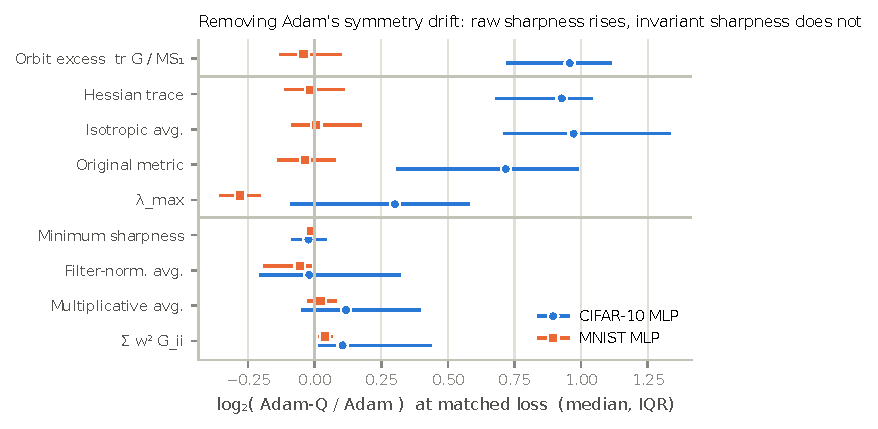
\includegraphics[width=0.75\linewidth]{fig3_intervention.pdf}
\caption{\textbf{Causal test.} Ratio of each measure for Adam-Q (Adam with its symmetry drift removed after every step) to Adam, for the same learning rate, batch size and seed at matched training loss (median and IQR over loss-matched checkpoint pairs). On CIFAR-10, removing the drift doubles the orbit excess and, with it, every raw trace-type measure. On MNIST, where the conserved coordinates are already close to the orbit minimum, the excess barely moves and neither do the raw measures. Invariant measures are unchanged in both cases.}
\label{fig:intervention}
\end{figure}

If the coordinate factor is caused by Adam's drift, removing the drift should change raw measures and leave invariant ones alone. \emph{Adam-Q} runs Adam and, after every step, applies the function-preserving rescaling that restores each unit's $Q_j$ to its initial value. This requires solving $c^2\|a_j\|^2-\|c_j\|^2/c^2=Q^{(0)}_j$ for $c>0$ in closed form. Adam's moment estimates are transformed covariantly: for a weight scaled by $s$, $m\mapsto m/s$ and $v\mapsto v/s^2$. Since the rescaling preserves the function, Adam-Q optimizes the same loss and differs from Adam only through Adam's lack of rescaling-equivariance. We rerun the 18 Adam configurations of each main sweep with Adam-Q and compare checkpoints of the same configuration whose training losses agree to within $25\%$ (73 of 78 pairs on CIFAR-10).

In 12 of the 18 CIFAR-10 configurations (base learning rate $10^{-4}$, and all runs at batch size 512) Adam-Q trains like Adam, reaching every loss target in the same or slightly fewer epochs. In the six noisiest configurations (base rate $3\times10^{-4}$ at batch sizes 32 and 128), however, Adam-Q stalls. It reaches loss $0.1$ two to three times later than Adam and never gets below $\approx0.05$ within 300 epochs, whereas Adam reaches $0.01$ by epoch $\approx55$. On MNIST all 18 Adam-Q runs train normally. So the drift is not merely a measurement nuisance: in noisy regimes it appears to help Adam train. Three controls, each run with two seeds at the three base settings, narrow this down. First, restoring $Q_j$ only every 50 steps instead of every step still stalls at batch sizes 32 and 128, so the stall is not caused by intervening at every step. Second, restoring $Q_j$ in only one hidden layer trains normally. Freezing just the first layer, which has fan-in 3072 and the largest drift, reaches loss $0.01$ in 57--78 epochs; freezing just the second takes 52--62, against 52--67 for Adam. The obvious hypothesis, that Adam must inflate its high-fan-in weights to shrink their relative step $\eta/|w_i|$, is therefore wrong: the stall appears only when both layers are prevented from drifting. Third, restoring $Q_j$ \emph{without} transforming Adam's moment estimates stalls at every batch size, including 512. That version is a harsher intervention rather than a cleaner control, which is why the covariant transformation is part of Adam-Q. Why the joint drift matters for optimization remains open. All comparisons below use only checkpoint pairs that are genuinely loss-matched. Across them, test accuracy at matched loss differs by a median factor of $0.995$. Adam-Q's coordinates stay SGD-like: first-layer imbalance falls from $0.89$ to $0.13$ and the orbit excess rises from $1.18$ to $2.35$. Figure~\ref{fig:intervention} shows the consequence on CIFAR-10. Every raw trace-type measure roughly doubles: $\tr G$ by a median factor of $1.91$ (IQR $1.63$--$2.04$), the isotropic average by $1.96$ and the original metric by $1.64$. The invariant measures are essentially unchanged: $\MS_1$ $0.98$ (IQR $0.94$--$1.03$), $\MS_{1/2}$ $0.99$, multiplicative $1.09$, and the partially invariant filter-normalized measure $0.99$. $\lambda_{\max}$ moves less ($1.23$, IQR $0.94$--$1.49$), consistent with its weaker dependence on the coordinate factor (\S\ref{sec:audit}). Ranked against SGD, Adam-Q is no longer rated flatter: $P(\text{flatter than SGD})$ by $\tr G$ drops from $0.64$--$0.75$ (Adam) to $0.21$--$0.35$ (Adam-Q), and by the original metric from $0.62$--$0.67$ to $0.12$--$0.34$. Minimum sharpness gives the same verdict for both ($0.06/0.01/0.22$ vs.\ $0.00/0.02/0.21$ at losses $0.3/0.1/0.01$; at $0.01$ only the 12 Adam-Q configurations that reach it are included). The one deviation is at the lowest loss target ($0.01$), where the median $\MS_1$ ratio is $0.88$. There, small residual differences between the two trajectories matter because cross-entropy curvature scales with the loss.

On MNIST the intervention changes little, which is what the decomposition predicts. MNIST's conserved coordinates happen to lie close to the orbit minimum (initial excess $1.79$ vs.\ $3.66$ on CIFAR-10), so Adam-Q's excess ($1.11$--$1.36$ across loss targets, median $1.17$) stays near Adam's ($1.21$). The raw measures accordingly move by at most about $13\%$ (median $\tr G$ ratio $0.88$--$1.07$ across targets), and the invariant measures are again unchanged ($\MS_1$ $0.99$, IQR $0.98$--$1.00$; $\MS_{1/2}$ $0.99$). Together the two datasets give a dose--response: Adam-Q moves raw sharpness in proportion to how far it moves the coordinates ($\times1.9$ when the excess doubles on CIFAR-10, about $\pm10\%$ when it barely changes on MNIST), and moves minimum sharpness in neither case. Only $\lambda_{\max}$ behaves differently on MNIST ($\times0.82$), a reminder that it is not rescaling-invariant either.

\subsection{Are Adam's coordinates good coordinates for SGD?}\label{sec:teleport}
If Adam ends near the trace-minimizing point and SGD does not, would SGD benefit from being moved there? Symmetry teleportation makes this cheap to test \citep{zhao2022teleport,zhao2024improving}, since our target has a closed form. Every 100 steps we map SGD (or SGD+M) to the minimum-sharpness point of its current orbit, computed from $\mathrm{diag}(G)$ on 1024 training examples, and transform the momentum buffer covariantly. We use four learning rates per optimizer and two seeds on the CIFAR-10 MLP.

It does not help; it destabilizes training. Ten of the 16 teleported runs diverged, against none of the 16 plain runs. At $\eta=0.12$, for instance, plain SGD reaches loss $0.01$ in 52--53 epochs, while both teleported runs diverge. The two teleported runs that did reach loss $0.01$ generalized worse (test accuracy $0.392$--$0.396$ vs.\ $0.433$--$0.441$).

The reason is the top eigenvalue. Logging $\lambda_{\max}$ around every teleport of an $\eta=0.12$ run, each teleport \emph{raised} it by 3--20\%, leaving it within 5\% of, or above, SGD's stability threshold $2/\eta=16.7$ in 8 of 11 teleports. SGD on its own keeps $\lambda_{\max}$ just below $2/\eta$, the self-stabilization of gradient descent at the edge of stability \citep{cohen2021eos,damian2023selfstabilization}, and the teleports keep knocking it over. The teleport scales were mild ($0.95$--$2.5$), so this is not an artifact of extreme rescalings. Measured on the converged networks, the same map \emph{lowers} $\lambda_{\max}$ (e.g.\ $15.9\to11.0$), so the trace and the top eigenvalue are minimized at different points of the orbit, and which point is ``better'' depends on what the optimizer needs. Adam's preferred coordinates are good for Adam, not for SGD.

\subsection{Long horizons: the orbit as a testbed for implicit sharpness regularization}\label{sec:labelnoise}
\begin{figure}[t]
\centering
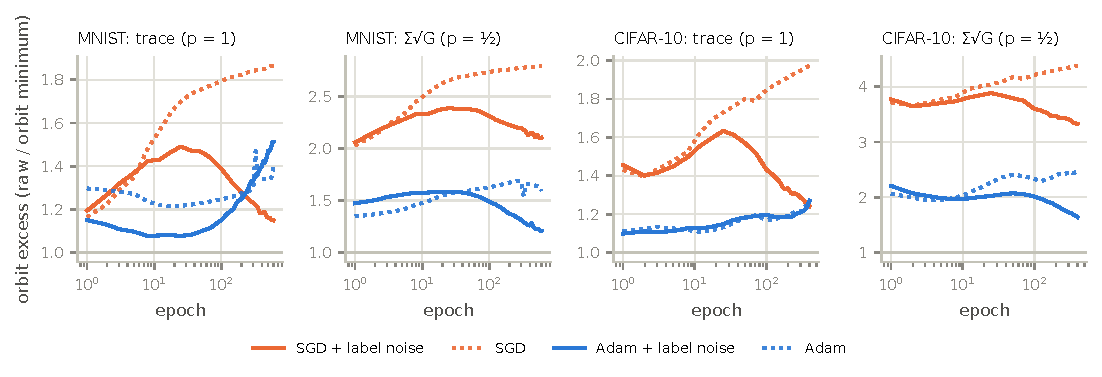
\includegraphics[width=\linewidth]{fig7_labelnoise.pdf}
\caption{\textbf{Where each optimizer drifts on long horizons.} Orbit excess for the trace ($p=1$) and for $\sum_i\sqrt{G_{ii}}$ ($p=\tfrac12$) during 600 (MNIST) and 400 (CIFAR-10) epochs, with and without label noise (SGD $\eta=0.12$, Adam $\eta=6\times10^{-4}$, batch size 128; mean of two seeds; log-scaled epoch axis). Without label noise SGD's coordinates freeze once the data are fit. With label noise SGD moves toward the trace-minimizing point, and Adam moves toward the $\sum_i\sqrt{G_{ii}}$-minimizing point while its trace excess grows: the destinations predicted for label-noise SGD \citep{blanc2020implicit,damian2021label} and for Adam \citep{li2025adam}.}
\label{fig:labelnoise}
\end{figure}

The two-phase picture makes predictions that ordinary training cannot test, because the slow phase needs persistent gradient noise and long horizons. Implicit-regularization theory supplies the standard device for this: \emph{label noise}, in which every label is replaced by a uniformly random class with probability $0.2$, freshly at every step \citep{blanc2020implicit,damian2021label}. We train the MLPs for 600 (MNIST) and 400 (CIFAR-10) epochs with SGD ($\eta\in\{0.06,0.12\}$) and Adam ($\eta\in\{2,6\}\times10^{-4}$), with and without label noise, two seeds each (32 runs), and track the orbit excess for $p=1$ and $p=\tfrac12$ (Fig.~\ref{fig:labelnoise}). Both targets are computable exactly. To our knowledge, the predictions of \citet{damian2021label} and \citet{li2025adam} had so far been checked only in diagonal linear networks and matrix factorization. The rescaling orbit gives a direction in a nonlinear network along which the predicted destination is known in closed form.

\textbf{Fast phase.} From an orbit excess of about $3.7$ at initialization, Adam reaches $1.09$--$1.13$ by epoch 5 on CIFAR-10 in all four Adam settings, while SGD is at $1.45$--$1.63$.

\textbf{Without noise, SGD freezes.} SGD's excess rises while the data are being fit and then stops changing once gradients vanish ($1.78$--$1.86$ on MNIST, $1.97$--$2.67$ on CIFAR-10).

\textbf{With label noise, SGD moves toward minimum trace.} After the initial transient its trace excess falls steadily: on CIFAR-10 from $2.05$ (epoch 25) to $1.63$ at $\eta=0.06$, and from $1.63$ to $1.24$ at $\eta=0.12$; on MNIST from $1.65$ (epoch 100) to $1.35$, and from $1.39$ to $1.15$. The movement is faster at the larger learning rate, as a second-order drift should be. Its per-unit curvature balance at $p=1$ shrinks markedly (CIFAR-10, $\eta=0.12$: mean $|\log A_j/B_j|$ from $1.37$ to $0.80$), while balance at $p=\tfrac12$ barely changes ($2.31$ to $2.04$).

\textbf{With label noise, Adam moves toward minimum $\sum_i\sqrt{G_{ii}}$.} At $\eta=6\times10^{-4}$, Adam's $p=\tfrac12$ excess falls (MNIST $1.56\to1.21$, CIFAR-10 $1.99\to1.64$) while its trace excess \emph{rises} (MNIST $1.10\to1.51$, CIFAR-10 $1.11\to1.27$).

\textbf{A per-run test.} For each run we compare the change in log excess from epoch 100 to the end at $p=\tfrac12$ with that at $p=1$. In all 8 label-noise SGD runs the trace excess falls by more (mean difference $+0.090$), and in all 8 label-noise Adam runs the $\sum\sqrt{G}$ excess falls by more (mean $-0.219$); a two-sided sign test gives $p=0.008$ for each. Each optimizer thus drifts toward the orbit point favoured by its own implicit regularizer. The ordinary-training regime of \S\ref{sec:audit} corresponds to the end of the fast phase, before this slow drift has had time to act.

\begin{figure}[t]
\centering
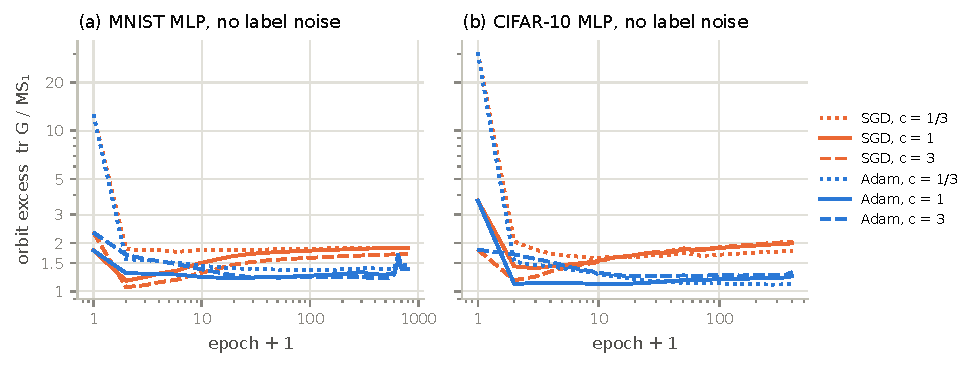
\includegraphics[width=0.9\linewidth]{fig9_memory.pdf}
\caption{\textbf{Coordinate memory.} The same initial function started at three points of its orbit (first-layer weights $\times c$, second layer $\div c$), trained without label noise (mean of two seeds). The initial spread in orbit excess disappears within one epoch for both optimizers, but from every starting point Adam ends below SGD.}
\label{fig:memory}
\end{figure}

\textbf{Does the starting orbit point matter?} Our account of SGD's excess leans on its conservation law, so we tested it directly. We start the \emph{same initial function} at three points of its orbit, multiplying the first layer's incoming weights and biases by $c\in\{\tfrac13,1,3\}$ and dividing the second layer's weights by $c$, and train with SGD and Adam, with and without label noise, for 800 (MNIST) and 400 (CIFAR-10) epochs (same learning rates as above, two seeds; 48 runs). The initial excess differs by a factor of $7.0$ (MNIST) and $16.9$ (CIFAR-10) across $c$ (Fig.~\ref{fig:memory}).\footnote{The CIFAR-10 runs of this experiment were done on a machine that could not reach the original CIFAR-10 host. We used a lossless PNG copy, whose ordering differs, so their 10k training subset differs from that of the other CIFAR-10 experiments.}

The prediction that SGD would remember its starting point in the orbit excess fails, and the reason is informative. For every optimizer, the spread across $c$ collapses to $1.3$--$1.9\times$ within the first epoch and ends at $1.03$--$1.19\times$ (one exception: $1.38\times$ for Adam with label noise on CIFAR-10). The curvature redistribution of early training, not the starting coordinates, sets the excess. SGD does remember its starting point in \emph{parameter} space: without label noise it keeps $90$--$99\%$ of the initial separation in mean first-layer $Q_j$ between $c=3$ and $c=\tfrac13$, and with label noise $79$--$83\%$. Adam does not erase that separation either. It enlarges it, to $1.5$--$2.0\times$ in seven of eight runs (and $0.97\times$ in one), consistent with a drift proportional to the units' $\ell_1$ norms (Remark~\ref{rem:fanin}). What does not depend on the starting point is the gap between the optimizers. Without label noise Adam ends at an excess of $1.29$--$1.51$ on MNIST and $1.09$--$1.35$ on CIFAR-10 from every starting point, against $1.71$--$1.89$ and $1.78$--$2.04$ for SGD. Starting SGD at a low excess does not keep it there (CIFAR-10, $c=3$: $1.82\to2.03$). Adam's low excess is therefore not an accident of the default initialization, and SGD's higher excess is where its own dynamics lead from any of these starting points.

The slow phase replicates across starting points. In the per-run test above (epoch 100 to the end), SGD's trace excess falls by more than its $\sum_i\sqrt{G_{ii}}$ excess in all 12 label-noise runs, and Adam's $\sum_i\sqrt{G_{ii}}$ excess falls by more in all 12 (sign test $p=0.0005$ each).

\textbf{Per-unit drift direction.} Between consecutive snapshots we correlate each hidden unit's change in $Q_j$ with its curvature imbalance $\log(A_j/B_j)$ at $p=1$ and at $p=\tfrac12$ (Spearman over units, averaged over snapshot pairs). Drift toward balance at power $p$ predicts a positive correlation at that $p$. Adam's per-unit drift matches $p=\tfrac12$ better than $p=1$ in every run, window and setting (24 of 24 runs, early and late). With label noise, the late-phase correlation is $+0.49$ at $p=\tfrac12$ against $-0.06$ at $p=1$ on MNIST, and $+0.18$ against $-0.16$ on CIFAR-10. Without label noise Adam's units drift \emph{away} from trace balance ($-0.25$ and $-0.56$; negative in 12 of 12 runs), as expected if the first-order sign-descent term rather than curvature dominates. For SGD the unit-level picture is mixed. On MNIST with label noise the drift matches $p=1$ better ($+0.39$ vs.\ $+0.26$, 6 of 6 runs). On CIFAR-10 it correlates positively with both but more strongly with $p=\tfrac12$ ($+0.60$ vs.\ $+0.76$, 0 of 6 runs favour $p=1$), although at the orbit level the same runs move toward minimum trace. The Fisher $\approx$ Gauss--Newton step of our heuristic is the likely weak point here. We therefore regard the orbit-level destinations, which replicate in 40 of 40 label-noise runs across both experiments, as established, and the unit-level mechanism for SGD as only partly confirmed.

\subsection{Consequences for generalization prediction}\label{sec:generalization}
\begin{figure}[t]
\centering
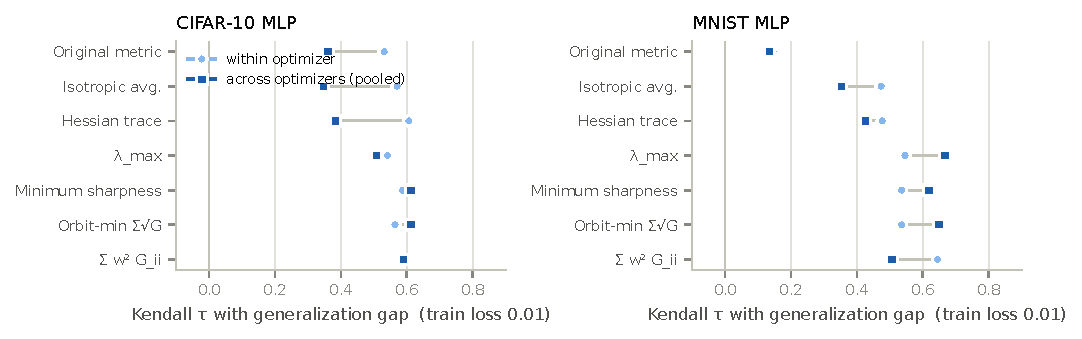
\includegraphics[width=\linewidth]{fig5_generalization.pdf}
\caption{Kendall $\tau$ between each measure and the generalization gap (train minus test accuracy) at training loss $0.01$, computed within each optimizer (averaged over the four optimizers) and pooled across optimizers. Raw measures lose predictive power when models from different optimizers are ranked together; minimum sharpness does not.}
\label{fig:gen}
\end{figure}

If the coordinate factor is a \emph{cross-optimizer} bias, it should hurt generalization prediction mainly when models from different optimizers are ranked together. This is what we find (Fig.~\ref{fig:gen}). Within one optimizer, raw $\tr G$ and $\MS_1$ predict the accuracy gap equally well (mean Kendall $\tau$ at loss $0.01$: $0.55$ vs.\ $0.59$ on CIFAR-10, $0.54$ vs.\ $0.54$ on MNIST). Pooled across optimizers, $\tr G$ drops to $0.38$ (CIFAR-10) and $0.47$ (MNIST), while $\MS_1$ stays at $0.61$ and $0.62$. The gain from removing the coordinate factor is larger on CIFAR-10 ($+0.21$ to $+0.23$ across loss targets) than on MNIST ($+0.01$ to $+0.15$), matching the smaller coordinate term there. The original metric is the weakest cross-optimizer predictor ($0.36$ on CIFAR-10, $0.14$ on MNIST). We use the accuracy gap rather than the test loss: at matched training loss in this memorization regime, the test loss is dominated by over-confident errors and is negatively correlated with most measures.

\subsection{Revisiting the original study}\label{sec:replication}
\begin{table}[t]
\centering
\small
\caption{The original protocol, re-run with five seeds: raw $[0,1]$ inputs, full training sets, 20 epochs, batch size 64, SGD $\eta=0.01$ vs.\ Adam $\eta=0.001$, measured once at the end (mean $\pm$ s.d.). The ``Adam is flatter'' result replicates. On CIFAR-10 it is almost entirely the coordinate factor; on MNIST it is a training-loss mismatch.}
\label{tab:replication}
\setlength{\tabcolsep}{5pt}
\begin{tabular}{lcccc}
\toprule
& \multicolumn{2}{c}{CIFAR-10} & \multicolumn{2}{c}{MNIST}\\
\cmidrule(lr){2-3}\cmidrule(lr){4-5}
& SGD & Adam & SGD & Adam\\
\midrule
Original metric $\Delta L/L$ (test) & $0.034\pm0.002$ & $0.012\pm0.003$ & $0.040\pm0.008$ & $0.014\pm0.010$\\
Training loss at measurement & $1.42\pm0.05$ & $1.29\pm0.02$ & $0.136\pm0.005$ & $0.008\pm0.004$\\
Test accuracy & $0.475\pm0.016$ & $0.496\pm0.005$ & $0.957\pm0.001$ & $0.978\pm0.002$\\
Hessian trace $\tr G$ & $1004\pm31$ & $395\pm19$ & $96.2\pm1.2$ & $9.7\pm3.1$\\
\quad minimum sharpness $\MS_1$ (function) & $353\pm18$ & $320\pm11$ & $72.0\pm1.1$ & $8.0\pm2.4$\\
\quad orbit excess $E$ (coordinates) & $2.85$ & $1.23$ & $1.34$ & $1.21$\\
Filter-normalized average, scale $0.1$ ($\times10^{4}$) & $78\pm34$ & $207\pm36$ & $41\pm9$ & $17\pm7$\\
Multiplicative average, $\sigma=0.1$ ($\times10^{4}$) & $109\pm21$ & $263\pm13$ & $61\pm13$ & $11\pm3$\\
\bottomrule
\end{tabular}
\end{table}

Table~\ref{tab:replication} re-runs the original fixed-epoch protocol with five seeds. The original result replicates: the relative perturbation metric is about $2.9\times$ lower for Adam on both datasets. The two datasets fail for different reasons, however. On \textbf{CIFAR-10}, both optimizers are far from convergence at similar training losses ($1.29$ vs.\ $1.42$). The $2.5\times$ gap in Hessian trace is almost entirely the coordinate factor ($E=1.23$ vs.\ $2.85$, i.e.\ $2.3\times$), the minimum sharpness is nearly equal ($320$ vs.\ $353$), and the invariant multiplicative measure and the partially invariant filter-normalized measure rate Adam about $2.5\times$ \emph{sharper}. On \textbf{MNIST}, after 20 epochs Adam has reached a $17\times$ lower training loss than SGD ($0.008$ vs.\ $0.136$), and every measure, invariant or not, is correspondingly lower. That is a loss-level confound of fixed-epoch comparisons, not a property of the optimizer, and matching the loss removes it (\S\ref{sec:audit}). One further detail of the original study may also have contributed. Its single Adam run on CIFAR-10 reported only $33.7\%$ test accuracy, against $49.6\pm0.5\%$ in our five-seed PyTorch replication. The difference may come from framework defaults (Keras uses Glorot initialization and $\epsilon=10^{-7}$) or from an unstable run. In our pilot runs with raw, uncentred inputs, Adam at $\eta=10^{-3}$ could oscillate around a training loss of $\approx1$. Either way, a high final loss lowers the relative metric $\Delta L/L$ mechanically.

\subsection{Convolutional networks}\label{sec:cnn}
\begin{figure}[t]
\centering
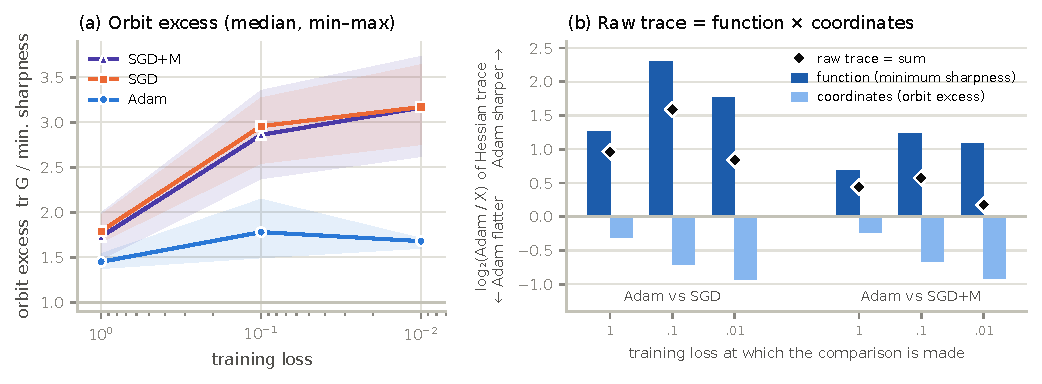
\includegraphics[width=\linewidth]{fig6_cnn.pdf}
\caption{\textbf{CNN on CIFAR-10.} \textbf{(a)} Orbit excess at matched training loss; rescaling acts on convolutional channels, through max-pooling and the flatten into the dense layer. \textbf{(b)} Exact split of the Adam/X trace ratio. On this network Adam's solutions are sharper at the function level, and the coordinate term, which again favours Adam and grows during training, hides most of that difference.}
\label{fig:cnn}
\end{figure}

We repeat the audit on the CNN with SGD, SGD+M and Adam (two learning rates each, batch size 128, three seeds; 18 runs). Rescaling now acts on whole channels, and minimum sharpness is computed from the exact per-sample $\mathrm{diag}(G)$ on 512 examples. Fifteen runs reached every loss target. The three Adam runs at the lower learning rate ($10^{-4}$) reached training loss $0.018$--$0.034$ by the 150-epoch cap, so comparisons at loss $0.01$ use only the other three Adam runs.

The mechanism carries over (Fig.~\ref{fig:cnn}a). Adam's channel imbalance is roughly twice SGD's in all three hidden layers (median $0.53/0.55/1.47$ vs.\ $0.22/0.35/0.65$ at loss $0.1$). Its orbit excess stays low at every loss level (median $1.45$, $1.78$, $1.68$ at losses $1$, $0.1$, $0.01$), while SGD's and SGD+M's grow from $1.7$--$1.8$ to $3.2$. The coordinate term again favours Adam and grows during training: $-0.31$ $[-0.38,-0.23]$, $-0.71$ $[-0.91,-0.49]$ and $-0.93$ $[-1.06,-0.79]$ bits against SGD, and $-0.24$ to $-0.91$ bits against SGD+M.

On this network, however, Adam's solutions are clearly sharper at the function level ($+1.27$ to $+2.30$ bits against SGD, $+0.68$ to $+1.24$ against SGD+M; all intervals exclude zero), and every invariant measure rates Adam sharper than both baselines ($P=0.00$ at every loss for $\MS_1$, multiplicative and $\sum_iw_i^2G_{ii}$), and so does the partially invariant filter-normalized measure. The coordinate factor therefore does not reverse the ranking here. It \emph{hides} part of the difference. Against SGD+M it hides most of it: the raw trace ratio is $+0.44$, $+0.57$ and $+0.18$ bits with intervals that include zero, and raw measures are inconclusive ($P=0.25$--$0.50$ for the trace and the original metric). A researcher using raw measures would conclude that Adam and SGD+M find equally flat minima on this CNN; an invariant measure shows Adam's are about $2\times$ sharper. Across the three settings, the same coordinate bias in Adam's favour thus reverses the ranking (CIFAR-10 MLP), flips it during training (MNIST MLP), or masks a large functional difference (CIFAR-10 CNN), depending on how large the functional difference is.


\subsection{Depth}\label{sec:depth}
\begin{figure}[t]
\centering
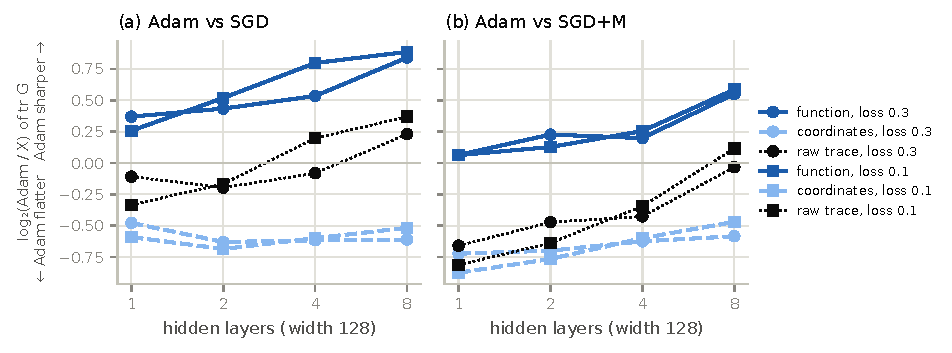
\includegraphics[width=0.85\linewidth]{fig10_depth.pdf}
\caption{\textbf{Depth.} Exact split~\eqref{eq:factor} of the Adam/X trace ratio for CIFAR-10 MLPs with 1--8 hidden layers of width 128 (three seeds each). The coordinate term is about the same at every depth; the function term grows with depth, so the coordinate factor reverses the raw ordering in shallow networks and masks the difference in deep ones.}
\label{fig:depth}
\end{figure}

Does the coordinate factor compound with depth, since every hidden layer adds its own rescaling symmetry? We train CIFAR-10 MLPs with $L\in\{1,2,4,8\}$ hidden layers of width 128 with SGD ($\eta=0.06$), SGD+M ($0.006$) and Adam ($6\times10^{-4}$), batch size 128 and three seeds (36 runs). All use He initialization with zero biases so that the signal is preserved at every depth, and all reached the targets $1$, $0.3$ and $0.1$.\footnote{These runs use the reordered CIFAR-10 copy described in \S\ref{sec:labelnoise}.} The answer is no (Fig.~\ref{fig:depth}). Adam's orbit excess stays at $1.16$--$1.39$ and SGD's and SGD+M's at $1.50$--$2.15$ at every depth. The coordinate term against SGD is $-0.48$ to $-0.74$ bits at every depth and target except the earliest target at depth 1 ($-0.15$), and against SGD+M it is $-0.47$ to $-0.88$ bits (again except the earliest target at depth 1, $-0.25$), a factor of $1.4$--$1.8$ in Adam's favour. What grows with depth is the function term: against SGD it rises from $+0.26$--$+0.37$ bits at depth 1 to $+0.76$--$+0.89$ at depth 8, and minimum sharpness rates Adam sharper than SGD in every pair at every depth ($P=0.00$). The consequence mirrors \S\ref{sec:audit} and \S\ref{sec:cnn} within one architecture family. At depths 1 and 2 the raw trace rates Adam flatter than SGD in every pair at losses $0.3$ and $0.1$ ($P=1.00$) while minimum sharpness rates it sharper in every pair ($P=0.00$): the ordering reverses. At depth 8 the raw trace rates Adam sharper as well, but by $+0.23$ to $+0.37$ bits instead of the $+0.84$ to $+0.89$ bits of the function term, so the coordinate factor hides most of the difference.

\subsection{Normalization layers and weight decay}\label{sec:bn}
\begin{figure}[t]
\centering
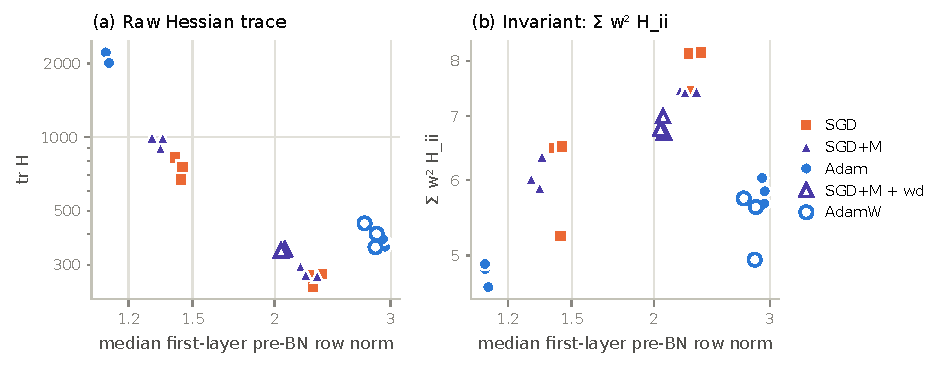
\includegraphics[width=0.85\linewidth]{fig8_bn.pdf}
\caption{\textbf{BatchNorm MLP on CIFAR-10} at training loss $0.1$ (one point per run). \textbf{(a)} The raw Hessian trace is almost a function of the pre-BN weight norm, which the learning rate sets; Adam at $3\times10^{-4}$ (left) looks sharpest and Adam at $10^{-3}$ (right) looks about as flat as SGD. \textbf{(b)} $\sum_iw_i^2H_{ii}$, invariant to every per-weight rescaling, does not follow the norm. It ranks every Adam run at $3\times10^{-4}$ below all twelve SGD and SGD+M runs without weight decay, and every Adam run at $10^{-3}$ below at least nine of them. Hollow markers: with weight decay.}
\label{fig:bn}
\end{figure}

BatchNorm adds a second symmetry. The loss is invariant to scaling each row of a pre-BN weight matrix, so the curvature with respect to that row scales as $1/\|w_{\mathrm{row}}\|^2$, and every optimizer moves along this symmetry: the gradient is orthogonal to a scale-invariant row, so even SGD grows its norm at second order, at a rate set by the learning rate \citep{vanlaarhoven2017l2,hoffer2018norm,arora2019autorate}. The ReLU rescaling survives between the BN affine parameters and the next layer. We test whether the coordinate factor still matters with the MLP of \S\ref{sec:protocol} with BatchNorm after each hidden linear layer (no bias before BN), trained on CIFAR-10 with SGD ($\eta\in\{0.1,0.3\}$), SGD+M ($\{0.01,0.03\}$), Adam ($\{3,10\}\times10^{-4}$), SGD+M with weight decay $5\times10^{-4}$ ($\eta=0.03$) and AdamW (weight decay $0.05$, $\eta=10^{-3}$), batch size 128 and three seeds (24 runs). All runs reached the targets $1$, $0.3$ and $0.1$, the last after a median of 35--44 epochs, and all are within $0.42$--$0.45$ test accuracy. The orbit-minimum machinery does not apply (BN couples the samples), so we compare raw measures with the measures that are invariant to every per-weight rescaling: $\sum_iw_i^2H_{ii}$ (Hutchinson), multiplicative average sharpness and ASAM. All measures use batch statistics.

\textbf{Raw measures read off the weight norm} (Fig.~\ref{fig:bn}). Across the 24 runs, the Hessian trace, $\lambda_{\max}$ and isotropic sharpness are strongly anticorrelated with the median first-layer pre-BN row norm (Spearman $\rho=-0.84$, $-0.76$, $-0.62$ for the trace at losses $1$, $0.3$, $0.1$). The invariant measures are not ($\rho$ between $-0.30$ and $+0.23$ for $\sum_iw_i^2H_{ii}$ and ASAM). The norms are set mostly by the learning rate. At loss $0.1$ the median first-layer row norm is $1.1$ for Adam at $3\times10^{-4}$ and $2.9$ at $10^{-3}$, against $1.3$--$1.4$ for SGD and SGD+M at their smaller rates and $2.2$--$2.3$ at their larger ones. Adam keeps its second-layer rows short at both rates ($0.61$ and $0.84$, against $0.95$--$1.71$ for SGD and SGD+M).

\textbf{The raw verdict depends on the learning-rate pairing; the invariant verdict does not.} Pooled over pairings, raw measures rate Adam \emph{sharper} than SGD ($P=0.25$ at every target for the trace, $\lambda_{\max}$ and isotropic sharpness; trace ratio $+0.38$, $+0.84$, $+1.00$ bits). Split by pairing, however, Adam at $3\times10^{-4}$ is rated flatter by the trace in $0$ of $9$ seed-and-target pairs against each of the four SGD and SGD+M settings, while Adam at $10^{-3}$ is rated flatter in $9/9$ against SGD at $\eta=0.1$ and SGD+M at $0.01$, in $4/9$ against SGD+M at $0.03$, and in $0/9$ against SGD at $0.3$ (22 of 72 pairs overall). The invariant measures rate Adam \emph{flatter} in every pairing: $\sum_iw_i^2H_{ii}$ in $70/72$ pairs (at least $8/9$ per pairing), ASAM in $72/72$ and multiplicative sharpness in $64/72$. Pooled, $P(\text{Adam flatter than SGD})$ is $1.00$, $1.00$, $0.92$ for $\sum_iw_i^2H_{ii}$ ($-0.27$ to $-0.47$ bits) and $1.00$ at every target for ASAM, with the same picture against SGD+M ($0.92$--$1.00$). Filter-normalized sharpness, which is invariant to the BN row scaling but not to the BN-affine rescaling, is inconclusive ($P=0.42$--$0.67$). With BatchNorm the coordinate factor therefore again reverses the ordering, but now in the \emph{opposite} direction to the plain MLP: raw measures understate Adam's flatness, because raw curvature is dominated by learning-rate-dependent weight norms rather than by Adam's ReLU-orbit drift. That invariant measures rate Adam flatter here, and sharper on the plain MLP and the CNN, is a further reason not to read our results as a statement about which optimizer finds flatter minima in general.

\textbf{Weight decay.} At the strengths used here, weight decay has little effect before loss $0.1$. Compared at the same learning rate, AdamW and Adam have almost the same first-layer norms ($2.85$ vs.\ $2.94$ at loss $0.1$) and raw traces ($+0.04$ to $+0.11$ bits), and SGD+M with weight decay has slightly shorter rows than without ($2.06$ vs.\ $2.23$) and a correspondingly higher raw trace ($+0.07$ to $+0.30$ bits) and slightly lower $\sum_iw_i^2H_{ii}$ ($-0.08$ to $-0.12$ bits; three pairs each). AdamW is rated flatter than SGD+M with weight decay by $\sum_iw_i^2H_{ii}$ and ASAM in all three pairs at every target, while the raw trace again depends on the target ($P=1.00$, $0.33$, $0.00$). Stronger weight decay and longer horizons, where the norm equilibrium of \citet{vanlaarhoven2017l2} is reached, remain to be tested.

%===============================================================================
\section{Discussion and limitations}
%===============================================================================
\textbf{Recommendations.} (i) Compare optimizers at matched training loss, not after a fixed number of epochs. (ii) Report at least one rescaling-invariant measure. Minimum sharpness is cheap given $\mathrm{diag}(G)$, and the orbit excess $E$ directly quantifies how much a raw trace comparison owes to the coordinates. (iii) Do not rely on canonicalizing to the minimum-norm point. (iv) Use a sanity check such as SAM versus its base optimizer: a measure that cannot tell them apart should not be used to rank optimizers.

\textbf{What we do and do not claim.} We do not claim that Adam's minima are universally sharper. Invariant measures can disagree with each other (\S\ref{sec:audit}), and sharpness depends strongly on the learning rate. We claim that raw-coordinate flatness comparisons between Adam and SGD-type methods contain an optimizer-dependent coordinate factor, that the factor has a precise mechanism (first-order drift along rescaling orbits, absent for SGD), and that it is large enough to reverse conclusions.

\textbf{Limitations.} The experiments are small: MLPs and a small CNN on 10k-example subsets, trained on a CPU. Our theory covers only the ReLU rescaling symmetry. With BatchNorm (\S\ref{sec:bn}) raw measures are dominated by a second, learning-rate-driven scale symmetry, and our weight-decay strengths and horizons were too small for weight decay to matter; larger normalized networks and stronger weight decay remain to be studied. The learning-rate grids are broad but finite. Our explanation of \emph{why} Adam's drift ends near minimum sharpness is a heuristic. Finally, the Adam-Q stalls in noisy regimes raise a question we do not answer: is the symmetry drift part of \emph{why} Adam works, for instance by adapting per-weight relative step sizes through the norms, rather than a side effect?

\section{Conclusion}
A well-known theoretical caveat, that sharpness depends on the parameterization, has a concrete and systematic practical consequence. Adam breaks the rescaling conservation law that SGD obeys, drifts at a rate $\propto\eta\sqrt{\text{fan-in}}$, and holds its solutions near the flattest representation on their symmetry orbits. The resulting coordinate factor can reverse, flip or mask optimizer flatness rankings, and it weakens sharpness--generalization correlations across optimizers. With BatchNorm a second, learning-rate-driven scale symmetry takes over and biases raw comparisons in the opposite direction. Invariant measures remove both. Beyond measurement, the rescaling orbit is a useful probe of optimizer dynamics: it separates a fast, first-order drift of adaptive methods from a slow, noise-driven drift whose destination differs between SGD and Adam exactly as implicit-regularization theory predicts.

\paragraph{Code and data.} All code, configurations and per-run results (training curves and all measures at every checkpoint) are available at \url{https://github.com/Ashvinj2004/LossLandscape-Research}.

\bibliographystyle{plainnat}
\bibliography{refs}

\appendix
\section{Measure definitions}\label{app:measures}
All measures use mean cross-entropy on a fixed evaluation subset of 4096 training examples (CNN: 1024; $\mathrm{diag}(G)$ for the CNN uses its first 512), shared by all models. Random perturbations use common random numbers across models.
\begin{itemize}[leftmargin=1.2em,itemsep=1pt]
\item \emph{Original metric}: $\big(\mathbb{E}_\varepsilon L_{\mathrm{test}}(w+\sigma\varepsilon)-L_{\mathrm{test}}(w)\big)/L_{\mathrm{test}}(w)$, $\varepsilon\sim\mathcal N(0,I)$ on all parameters, $\sigma=0.01$, 10 draws, full test set.
\item \emph{Isotropic average}: $\mathbb{E}L(w+\sigma\varepsilon)-L(w)$, $\sigma\in\{0.003,0.01,0.03\}$, 16 draws; we report $\sigma=0.01$.
\item \emph{Filter-normalized average} \citep{li2018visualizing}: each output unit's (or filter's) row of a Gaussian direction is rescaled to the norm of the corresponding weight row; biases are not perturbed; scale $\in\{0.01,0.03,0.1\}$, 16 draws; we report $0.03$. Invariant to scaling a row, not to neuron rescaling (\S\ref{sec:protocol}).
\item \emph{Multiplicative average}: $\delta=\sigma|w|\odot\varepsilon$, $\sigma\in\{0.01,0.03,0.1\}$; we report $0.03$.
\item \emph{Hessian trace}: Hutchinson with 20 Rademacher probes. $\tr G$: exact, from the exact diagonal Gauss--Newton matrix (which matches the Hessian trace closely at the loss levels studied).
\item $\lambda_{\max}$: Lanczos (\texttt{scipy eigsh}, tolerance $10^{-3}$) on Hessian--vector products.
\item \emph{SAM worst-case}: $\max_{\|\delta\|_2\le0.05}L(w+\delta)-L(w)$ by 10 steps of normalized projected gradient ascent with step $0.4\rho$. \emph{ASAM worst-case} \citep{kwon2021asam}: the same with $\|\delta/|w|\|_2\le0.5$.
\item $\MS_p$: coordinate descent until the relative change is below $10^{-10}$. The minimum-norm point: alternating per-unit balancing until $\max_j|\log c_j|<10^{-7}$.
\end{itemize}
Verification: the fast MLP $\mathrm{diag}(G)$ matches a per-sample implementation to $2{\times}10^{-8}$, which matches a brute-force $J^\top SJ$ to $3{\times}10^{-8}$. Rescalings preserve the network output to $3{\times}10^{-6}$. The analytic transport of $\mathrm{diag}(G)$ matches recomputation to $2{\times}10^{-7}$ (MLP) and $3{\times}10^{-7}$ (CNN). $\MS_p$ was never beaten by the raw, minimum-norm or random rescalings tested. Under random rescalings (log-scale s.d.\ $1$), the multiplicative average, ASAM and $\sum_iw_i^2H_{ii}$ change by less than $2{\times}10^{-4}$ relative (the residual comes from BatchNorm's $\epsilon$, which moves the loss itself by as much), both for ReLU neuron rescaling in the MLP and for the two symmetries of the BatchNorm MLP (\S\ref{sec:bn}); filter-normalized sharpness changes by factors of $9.5$ and $19$ under the neuron and BN-affine rescalings.

\section{Drift experiment: all optimizers}\label{app:drift}
\begin{table}[h]
\centering
\small
\caption{Drift experiment (CIFAR-10 MLP, $32{\times}32$ inputs, batch size 128, 20 epochs, mean of two seeds). $D^{(1)}$ and $D^{(2)}$ are the cumulative first- and second-order drift terms of~\eqref{eq:decomp}, averaged over first-layer units; $E$ is the final orbit excess. The decomposition closes to $\le1.3\times10^{-6}$ in every run.}
\label{tab:drift}
\begin{tabular}{llccccc}
\toprule
Optimizer & $\eta$ & final train loss & $D^{(1)}$ & $D^{(2)}$ & imbalance (L1) & $E$\\
\midrule
SGD & $0.01$ & 1.44 & $0.0000$ & 0.0023 & 0.31 & 1.70\\
SGD & $0.03$ & 0.92 & $0.0000$ & 0.064 & 0.32 & 2.31\\
SGD & $0.1$ & 0.57 & $0.0000$ & 0.577 & 0.47 & 1.78\\
SGD+M & $0.001$ & 1.45 & 0.0023 & 0.0001 & 0.31 & 1.68\\
SGD+M & $0.003$ & 0.90 & 0.048 & 0.0027 & 0.30 & 2.41\\
SGD+M & $0.01$ & 0.46 & 0.576 & 0.032 & 0.48 & 1.99\\
\midrule
Adam & $3{\times}10^{-5}$ & 1.50 & 0.067 & 0.0003 & 0.41 & 1.14\\
Adam & $10^{-4}$ & 1.13 & 0.255 & 0.0032 & 0.55 & 1.14\\
Adam & $3{\times}10^{-4}$ & 0.62 & 1.076 & 0.027 & 0.86 & 1.12\\
Adam & $10^{-3}$ & 0.27 & 6.151 & 0.261 & 1.40 & 1.19\\
RMSprop & $3{\times}10^{-5}$ & 1.37 & 0.114 & 0.025 & 0.48 & 1.11\\
RMSprop & $10^{-4}$ & 0.96 & 0.397 & 0.272 & 0.78 & 1.10\\
RMSprop & $3{\times}10^{-4}$ & 0.52 & 1.149 & 2.186 & 1.27 & 1.28\\
signSGD & $3{\times}10^{-5}$ & 1.57 & 0.052 & 0.0042 & 0.40 & 1.15\\
signSGD & $10^{-4}$ & 1.25 & 0.149 & 0.047 & 0.51 & 1.14\\
signSGD & $3{\times}10^{-4}$ & 0.81 & 0.359 & 0.423 & 0.78 & 1.14\\
\bottomrule
\end{tabular}
\end{table}
For sign descent and RMSprop at larger learning rates the second-order term becomes comparable to the first-order one. Each coordinate moves by $\approx\eta$, so $\|u_{a_j}\|^2-\|u_{c_j}\|^2\approx\eta^2(d_{\mathrm{in}}-d_{\mathrm{out}})$, which is a second, fan-in-driven contribution in the same direction.

\section{Robustness to the learning-rate pairing}\label{app:lrpairs}
\begin{table}[h]
\centering
\small
\caption{$P(\text{Adam rated flatter than SGD})$ for each pair of base learning rates, pooled over the $3\times3$ batch-size pairs, three seeds and training losses $\{0.1,0.03,0.01\}$ (81 pairs per cell).}
\label{tab:lrpairs}
\begin{tabular}{cc cccc cccc}
\toprule
& & \multicolumn{4}{c}{CIFAR-10} & \multicolumn{4}{c}{MNIST}\\
\cmidrule(lr){3-6}\cmidrule(lr){7-10}
Adam $\eta_0$ & SGD $\eta_0$ & $\tr G$ & orig. & $\MS_1$ & filter & $\tr G$ & orig. & $\MS_1$ & filter\\
\midrule
$10^{-4}$ & $0.01$ & 1.00 & 1.00 & 0.00 & 0.02 & 0.84 & 0.91 & 0.42 & 0.26\\
$10^{-4}$ & $0.03$ & 0.06 & 0.00 & 0.00 & 0.05 & 0.19 & 0.58 & 0.00 & 0.10\\
$3{\times}10^{-4}$ & $0.01$ & 1.00 & 1.00 & 0.27 & 0.05 & 0.98 & 0.93 & 0.88 & 0.54\\
$3{\times}10^{-4}$ & $0.03$ & 0.60 & 0.59 & 0.07 & 0.09 & 0.68 & 0.83 & 0.21 & 0.33\\
\bottomrule
\end{tabular}
\end{table}

\section{Calibration of learning rates}\label{app:calibration}
Before the main sweeps we trained every optimizer with four learning rates and three batch sizes for up to 200 epochs (seed 0, no measures). Table~\ref{tab:calib} reports the epoch at which the training loss first fell below $0.01$, or the final loss in parentheses if it did not. No single learning rate trains stably at every batch size: SGD at $\eta=0.1$, for example, fails at $B=32$ but works at $B=512$. We therefore use square-root scaling, $\eta=\eta_0\sqrt{B/32}$, with the base rates $\eta_0\in\{0.01,0.03\}$ (SGD), $\{10^{-3},3{\times}10^{-3}\}$ (SGD+M, SAM) and $\{10^{-4},3{\times}10^{-4}\}$ (Adam). Every main-sweep run reached all loss targets within 300 epochs.
\begin{table}[h]
\centering
\small
\caption{Calibration: epochs to reach training loss $0.01$ (final loss in parentheses if not reached in 200 epochs).}
\label{tab:calib}
\begin{tabular}{llccc@{\qquad}llccc}
\toprule
\multicolumn{5}{c}{CIFAR-10 MLP} & \multicolumn{5}{c}{MNIST MLP}\\
\cmidrule(lr){1-5}\cmidrule(lr){6-10}
Opt. & $\eta$ & $B{=}32$ & $128$ & $512$ & Opt. & $\eta$ & $B{=}32$ & $128$ & $512$\\
\midrule
SGD & 0.01 & 67 & (0.01) & (0.85) & SGD & 0.01 & 61 & (0.02) & (0.16)\\
SGD & 0.03 & 49 & 94 & (0.10) & SGD & 0.03 & 20 & 80 & (0.03)\\
SGD & 0.1 & (0.77) & 56 & 163 & SGD & 0.1 & 9 & 24 & 98\\
SGD & 0.3 & (2.30) & (0.79) & (1.23) & SGD & 0.3 & 19 & 10 & 35\\
SGD+M & 0.001 & 67 & (0.01) & (0.86) & SGD+M & 0.001 & 61 & (0.02) & (0.16)\\
SGD+M & 0.003 & 63 & 80 & (0.04) & SGD+M & 0.003 & 21 & 81 & (0.04)\\
SGD+M & 0.01 & (0.64) & 63 & 98 & SGD+M & 0.01 & 9 & 26 & 103\\
SGD+M & 0.03 & (2.29) & (0.50) & 75 & SGD+M & 0.03 & 20 & 11 & 36\\
SAM & 0.001 & 129 & (0.05) & (1.02) & SAM & 0.001 & 61 & (0.01) & (0.16)\\
SAM & 0.003 & 105 & 129 & (0.12) & SAM & 0.003 & 23 & 77 & (0.03)\\
SAM & 0.01 & (0.32) & 93 & 161 & SAM & 0.01 & 12 & 27 & 96\\
SAM & 0.03 & (1.60) & (0.23) & 106 & SAM & 0.03 & 13 & 12 & 35\\
Adam & 3e-5 & (0.02) & (0.41) & (0.91) & Adam & 3e-5 & 161 & (0.06) & (0.17)\\
Adam & 1e-4 & 97 & 164 & (0.13) & Adam & 1e-4 & 50 & 112 & (0.03)\\
Adam & 3e-4 & 60 & 81 & 158 & Adam & 3e-4 & 20 & 44 & 99\\
Adam & 1e-3 & (0.08) & 52 & 70 & Adam & 1e-3 & 16 & 18 & 38\\
\bottomrule
\end{tabular}
\end{table}

\section{Edge-of-stability observation}\label{app:eos}
In pilot runs with the original raw inputs (CIFAR-10 MLP, batch size 128), SGD's $\lambda_{\max}$ tracked the stability threshold $2/\eta$: $17$--$22$ at $\eta=0.1$ (threshold $20$), $47$--$74$ at $\eta=0.03$ ($67$), and $187$--$252$ at $\eta=0.01$ ($200$). Sharpness comparisons at a single learning rate per optimizer therefore largely compare learning rates.

\end{document}
